\chapter{誤差改善に向けた手法の検証}\label{chapt3}

\section{距離分解能と統計誤差の関係}
提案手法であるラマンDIALでは,
\ce{SO2}が高濃度, あるいは広範囲に分布する環境において測定を行う場合,
レーザ光およびラマン散乱光の減衰が大きくなり,
受信光子数の低下に伴って統計誤差が増大する.
そのため, \ce{SO2}濃度の変動による統計誤差の増大を考慮した
観測システムおよび信号処理手法の設計が不可欠である.

統計誤差を低減する手法として,
ライダー観測では信号加算による距離分解能の調整が一般に用いられる.
信号加算では, 計測時には距離分解能を細かく設定してライダー信号を取得し,
信号処理段階で隣接する複数距離の信号を加算することで,
その平均距離に対応する信号として扱う.
この処理により受信信号のS/Nは向上する一方,
複数距離の情報が統合されるため距離分解能は低下する.

そこで,
二酸化硫黄が豊富に存在する火山環境での観測を想定し,
信号加算の有無がラマンDIALによる測定性能に与える影響について
数値シミュレーションにより評価した.

霧島火山では,
三宅島と比較して3\sim4倍程度の二酸化硫黄濃度が報告されている.
これを参考に濃度分布を再設定した.
\cref{fig:gas_setting_SO2thick}に再設定した火山ガス濃度分布を示す.
\begin{figure}
  \centering
  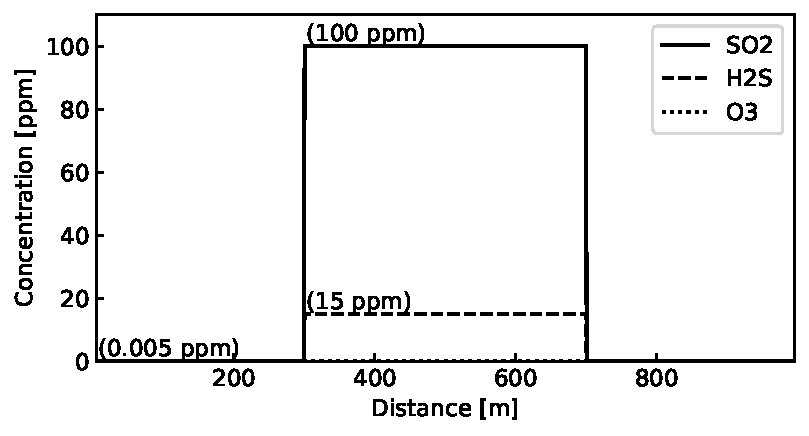
\includegraphics{fig/sim_02_1_env}
  \caption{\ce{SO2}が豊富な火山環境を想定した濃度分布設定}
  \label{fig:gas_setting_SO2thick}
\end{figure}

\noindent
\ref{chapt2}章で用いた設定から,
高濃度区間の\ce{SO2}濃度を\qty{100}{ppm}に変更している.
なお, システムパラメータは\ref{chapt2}章と同一である.

\cref{fig:fix_res}に,
距離分解能\qty{5}{m}のライダー信号から\ce{SO2}濃度を推定した場合と,
信号加算により距離分解能を\qty{25}{m}に調整した場合の
シミュレーション結果を示す.
\begin{figure}
  \centering
  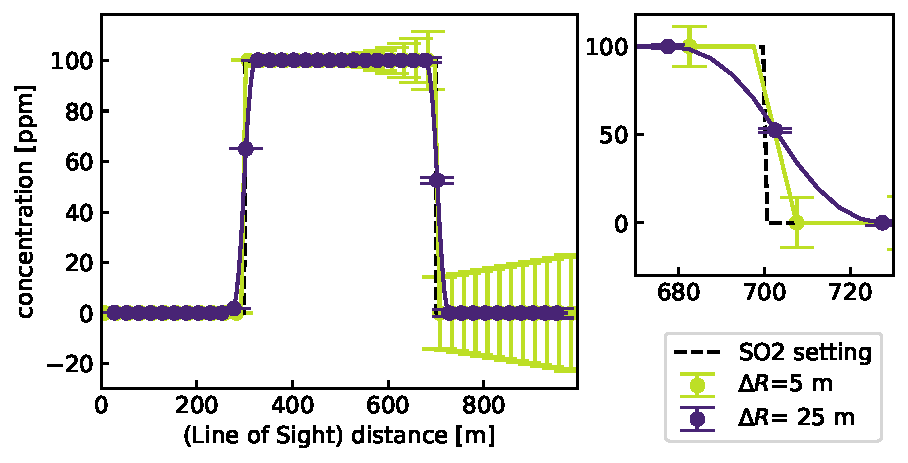
\includegraphics{fig/sim_02_1_dR-5mto25m.pdf}
  \caption{$\Delta R=5, 25 \unit{m}$による\ce{SO2}測定シミュレーション}
  \label{fig:fix_res}
\end{figure}

\noindent
横軸はライダーの視線距離, 縦軸は\ce{SO2}濃度である.
エラーバーは統計誤差を表す.
視線距離\qty{700}{m}付近の高濃度区間における測定点を比較すると,
$\Delta R=\qty{5}{m}$では\staterr が\qty{13.4}{ppm}であるのに対し,
$\Delta R=\qty{25}{m}$では\qty{1.2}{ppm}まで低減している.
一方, 実線で示す推定結果に注目すると,
$\Delta R=\qty{25}{m}$の場合には,
設定値（点線）に対する急峻な濃度変化への追従性が低下している.

\newpage
\cref{equ:stat_err}より,
統計誤差\staterr は距離分解能$\Delta R$と相反関係にあり,
信号加算によって高濃度ガスが滞留する区間における
急激な濃度変化を十分に捉えられなくなることが確認された.
信号加算前後の受信信号強度を\cref{fig:fix_power}に示す.
\begin{figure}
  \centering
  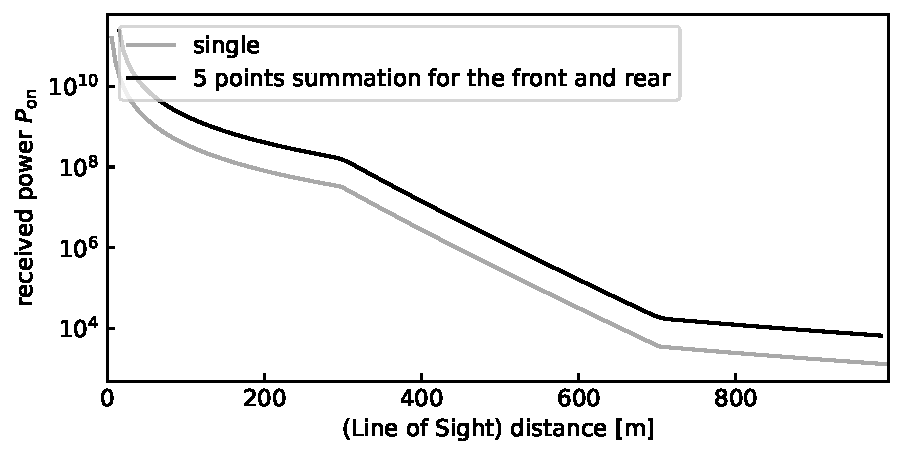
\includegraphics{fig/sim_02_1_power.pdf}
  \caption{信号加算前後の受信信号強度の変化}
  \label{fig:fix_power}
\end{figure}

\noindent
横軸は視線距離, 縦軸は受信光子数である.
単信号の信号強度を見ると,
\qty{300}{m}付近と\qty{700}{m}付近で減衰傾向が変化している.
これは, 低濃度区間では大気吸収が支配的であったのに対し,
高濃度区間では\ce{SO2}吸収が支配的となったためである.
このような信号強度の距離依存性を利用することで,
距離分解能が要求されない区間に限定して
信号加算を適用する手法が有効であると考えられる.

\newpage
\section{他ガス濃度推定による干渉誤差の補正効果}
\cref{equ:contam_err}より,
測定対象である\ce{SO2}以外の干渉ガス濃度$\subrm{n}{gas}$が高い場合,
干渉誤差\cntmerr は増大する.
\ref{chapt2}章で用いた\ce{H2S}濃度分布では,
高濃度区間の濃度を\qty{15}{ppm}としていた.
しかし, 霧島火山では\qty{100}{ppm}から\qty{2000}{ppm}程度の
\ce{H2S}濃度が報告されている.
このような環境では,
干渉誤差を無視できない可能性がある.

この場合,
干渉ガス濃度を事前に推定して\cntmerr を算出し,
\cref{equ:n_SO2}から差し引くことで,
干渉ガスの影響を低減できる.
そこで,
\ce{H2S}が豊富に存在する火山環境を想定し,
干渉誤差補正の有無が測定性能に与える影響を評価した.

\cref{fig:gas_setting_H2Sthick}に,
再設定した火山ガス濃度分布を示す.
高濃度区間の\ce{H2S}濃度を\qty{1000}{ppm}に変更している.
システムパラメータは\ref{chapt2}章と同一である.

\newpage
\begin{figure}
  \centering
  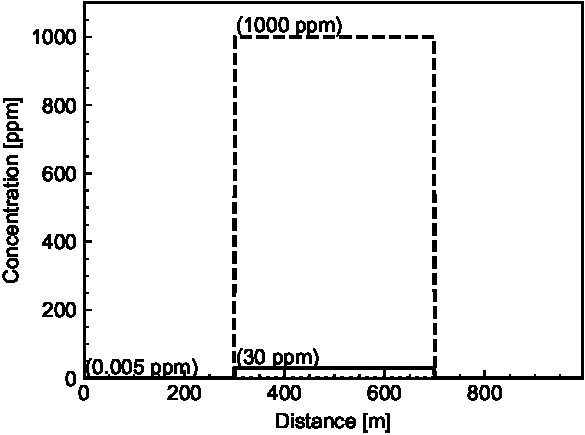
\includegraphics{fig/sim_02_2_env.pdf}
  \caption{\ce{H2S}が高濃度の火山ガス分布設定}
  \label{fig:gas_setting_H2Sthick}
\end{figure}

実観測を想定すると,
火口位置は目視等により概ね把握可能であり,
視線上で高濃度ガスが存在する区間を予測できる.
ここでは, 視線距離\qty{500}{m}に火口が存在し,
その前後\qty{100}{m}を高濃度区間と仮定した.

推定条件として, 次の5ケースを設定した.
\ce{O3}濃度は観測領域全域で\qty{0.005}{ppm}とした.
\begin{enumerate}[label=(\arabic*)]
  \item 無補正
  \item 大気および\ce{O3}を補正
  \item 大気, \ce{O3}, \qty{500}{ppm}の\ce{H2S}を補正
  \item 大気, \ce{O3}, \qty{600}{ppm}の\ce{H2S}を補正
  \item 大気, \ce{O3}, \qty{800}{ppm}の\ce{H2S}を補正
\end{enumerate}

\noindent
\cref{fig:corr_cntm}に各推定条件による
干渉補正後の\ce{SO2}濃度推定結果を示す.

\newpage
\begin{figure}
  \centering
  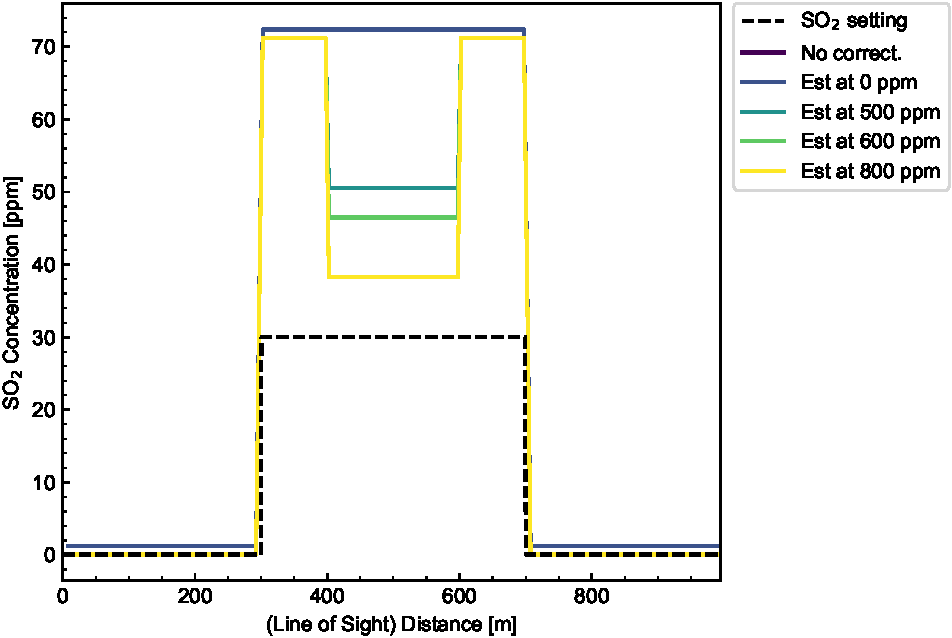
\includegraphics{fig/sim_02_2_contami_result.pdf}
  \caption{
    高濃度区間の一部について\ce{H2S}補正を行ったラマンDIALによる
    \ce{SO2}測定シミュレーション
  }
  \label{fig:corr_cntm}
\end{figure}

\noindent
補正量が大きいほど,
高濃度区間における\ce{SO2}濃度推定値は
設定値（点線）に近づく傾向を示す.
一方,
仮定した高濃度区間外である
\qty{300}{m}から\qty{400}{m},
および\qty{600}{m}から\qty{700}{m}では,
高濃度の\ce{H2S}による干渉誤差が顕著である.
干渉誤差の改善量を\cref{tab:res_cntm}に示す.
\begin{table}
  \centering
  \caption{各推定条件における\ce{SO2}濃度推定結果と濃度誤差}
  \label{tab:res_cntm}
  \begin{tabular}{ccc}
    \hline
    推定条件 & \ce{SO2}推定値 [\unit{ppm}] & 濃度誤差 [\unit{ppm}]\\
    (1) & 72.4  & 42.4\\
    (2) & 71.2  & 41.2\\
    (3) & 50.6  & 20.6\\
    (4) & 46.5  & 16.5\\
    (5) & 38.2  & 8.24\\
    \hline
  \end{tabular}
\end{table}

\noindent
大気および\ce{O3}のみを補正した場合でも,
干渉誤差は約\qty{1}{ppm}低減している.
さらに,
\ce{H2S}濃度を\qty{800}{ppm}と仮定した場合には,
干渉誤差は\qty{8.24}{ppm}まで低減した.
しかし,
設定した\ce{SO2}濃度が\qty{30}{ppm}であることを考慮すると,
十分な測定精度が得られているとは言い難い.
以上より,
干渉ガス濃度が非常に高い環境での測定は困難であることが示された.
実観測では,
干渉ガス濃度が比較的安定した火山で事前に妥当な推定値を設定する,
あるいは他手法による補助的な濃度測定と併用する必要がある.

\newpage
\section{信号加算と干渉ガス補正による効果}
本章の結論として, 
ライダー信号の処理による統計誤差の抑制について, 
$\Delta R$ を\qty{5}{m}から\qty{25}{m}として処理することで
\ce{SO2}が\qty{100}{ppm}の高濃度領域で発生する統計誤差を, 
\qty{13.4}{ppm}から\qty{1.2}{ppm}まで抑制できる. 
しかし, 濃度分布に対する追従性が悪化するため, 
信号強度の距離変化に合わせて距離分解能が要求されない区間で信号加算を行うといった柔軟な測定が有効だといえる. 
また, ラマンDIAL推定時の干渉ガス濃度の推定による補正について, 
霧島火山のような\ce{H2S}高濃度地点の測定をする際は, 
干渉誤差も濃度に従って大きくなり,
補正が困難となるため, 
事前に妥当な推定値を用意するか, 
補助的な濃度測定手法を併用する必要があることが明らかとなった. 
